\section{Motivation}

Digital signal processing has over the last 100 years gone from almost non-existent to utmost critical importance. By processing signal data, one can get access to all kinds of information, music, movement and locations. There are tons of different devices for recording signals from the environments. From more well known ones such as microphones and sensors, to less commercial technologies. \\

\begin{figure}[ht]
    \centering
    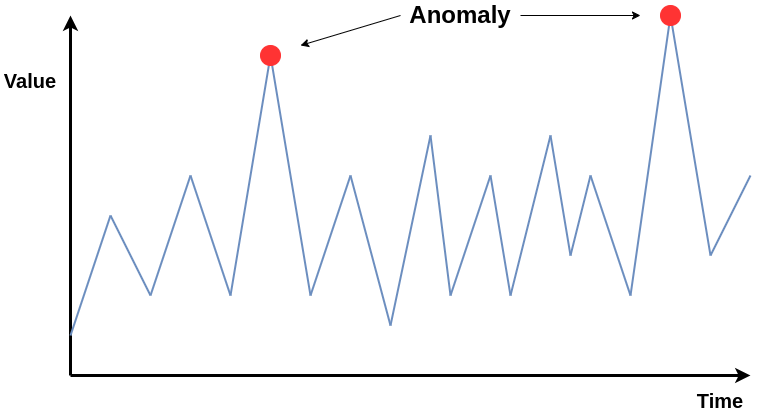
\includegraphics[scale=0.4]{figures/anolay_line.png}
    \label{fig:anomaly_example}
\end{figure}

The world of digital signal processing is nothing new to academia, and computer science in general. Some of the most magnificent and trailblazing algorithms, like the \acrfull{dft} algorithm revolve around solving problems revolving around these data. With more and more sensors being used around us, as well as the increasing amount of data stored, the larger the need for processing and interpreting this data has become. 
\acrfull{das} is a rather new technology that allows for real-time analysis over fiber-optical cables, and gives us highly sensitive senor data to work with. \acrshort{das} has gained more recognition. \\

It is hard to underestimate the impact \acrshort{ai} has had upon the general population this last couple of years. Ever since OpenAI released ChatGPT the 30th of november 2022 \cite{chatgpt} the amount of \acrshort{ai} technology and applications has exploded, not only large language models (\acrshort{llm}), but other domains have garnered attention as well. \acrshort{llm}s made \acrfull{rnn} more popular than they had been for a while. These models are good at remembering information, making current desicions based on previous ones. \\ 

\acrshort{das} technology in itself has now started garnering attention for research, and several papers have previously studied  how one can process this data. \acrshort{ai} and \acrshort{ml} models have been constructed for looking at time series data, and analyzing sensor data, although several of theses have studied .  Only recently has \acrshort{ai}

Anomaly detection on \acrshort{das} data 

Unsupervised learning has in later years returned after the explosion of generatiive models. They are well suited for detecting novel anomalies \cite{wei2022lstmautoencoder} \cite{srivastava2016unsupervised} and do not require labeling of data, something that can rather dificult on DAS data. Both GANs, AE, and LSTM VAE have been proven to have good metrics for determining anomalies. 


Python has for a long been the \textit{de-facto standard} language both for \acrshort{ai}, \acrshort{ml} and data analysis. All kinds of heavy pre-processing of data before training the data is being written in C or C++ or other more performant languages.    




Previous work on this data (see \cite{projthesis}) revolved around processing \acrshort{hdf5} files as fast and efficient as possible, trying to parallellize already existent code, and take advantage of newer technologies, such as Julia.

\subsection{NTNU SFI Center for Geophysical Forecasting}



We hereby present \texttt{JudasNET}, a LSTM VAE network written in Julia for anomaly detection on \acrshort{das} data. Additionally, we present \texttt{Judas - (Julia \& DAS)}, a Julia package containing functions for parsing HDF5 files, signal processing methods specifically for DAS sensor data, as well as functions for training, inference and utilities for AI models related to DAS data. As a sideeffect, we also show how Julia can be used effectively within multiple different fields to enable , and be easily tuned to their needs,